\documentclass[11pt]{article}

\usepackage[margin=1in]{geometry}
\usepackage{amsmath,amssymb}
\usepackage{graphicx}
\usepackage{hyperref}
\usepackage{booktabs}
\usepackage{natbib}
\usepackage{xcolor}

\newcommand{\pending}[1]{\textcolor{red}{\textbf{[PENDING RESULTS: #1]}}}

\title{Does Recursive Computation Pay Off Under Delay?\\
Testing a Complexity-Scaling Hypothesis for Tiny Recursive Policies\\
in Model-Free Control}
\author{}
\date{Draft --- Phase 1 complete (48/48 runs); awaiting author review before Phase 2}

\begin{document}
\maketitle

\begin{abstract}
Tiny Recursive Models (TRM) trade parameter count for iterative, weight-tied computation, and have recently been applied to control as a learned corrector that refines a control sequence or trajectory against \emph{known} dynamics \citep{jainlinares2025trc, wijayatunga2026trmpl}. We study a mechanistically different use of the same architecture: recursion as an \emph{implicit memory / state-estimation} mechanism inside \emph{model-free} reinforcement learning under action delay, where the environment's dynamics are never modeled and the only signal available is a stream of sampled transitions. A pilot on Pendulum-v1 found a TRM-trunk actor/critic, a transformer-trunk actor/critic, and a memoryless DNN [256,256] actor/critic converge to comparable reward under 1-step delay, with TRM costing roughly 18x the wall-clock training time of the DNN. Rather than conclude TRM's recursive mechanism is unhelpful for delay-robust control, we treated this as evidence that Pendulum-v1 may be too simple a partially-observable task to stress any architecture's memory capacity, and tested the falsifiable, pre-registered hypothesis that TRM's relative disadvantage shrinks (or reverses into an advantage) once task complexity --- operationalized as episode horizon and reward sparsity --- crosses a specific, stated threshold. We compared four trunks (DNN, Transformer, TRM, and an LSTM mechanistic control) on Pendulum-v1 and MountainCarContinuous-v0 (a $\sim$5x longer-horizon, sparse-reward task), under 0-step and 1-step delay, 3 seeds per condition (48 runs total), reporting reward, wall-clock training time, and parameter count as co-equal metrics. \textbf{Full-data replication on Pendulum-v1 found TRM significantly \emph{worse} than DNN (6/6 seed-pairs, one-sided sign test $p=0.016$), not merely tied --- a materially different picture than the informal pilot suggested. On MountainCarContinuous-v0, that gap closed to a statistical tie (3/6 pairs, $p=0.66$ vs.\ DNN; 4/6 pairs, $p=0.34$ vs.\ Transformer): directionally consistent with the pre-registered threshold prediction, but not significant at this sample size.} The specific horizon/sparsity threshold tested is therefore falsified as a source of a \emph{significant} TRM advantage, though the direction of movement does not rule out the general hypothesis at a higher complexity rung (Phase 2, not yet run). TRM's wall-clock overhead over DNN meanwhile \emph{grew} with complexity (7.0x on Pendulum to 14.1x on MountainCarContinuous), so its cost scaled up at least as fast as any undetected benefit.
\end{abstract}

\section{Background}

\subsection{Delay in continuous control}

Real control systems rarely observe and act instantaneously: actuation, sensing, and computation all introduce delay. In a standard (undelayed) Markov Decision Process (MDP), the current observation is a sufficient statistic for predicting the next state and reward given the current action. Delay breaks this: the reward and next observation actually experienced at time $t$ were caused by an action chosen $d$ steps earlier, not the action chosen ``now'' --- the raw observation is no longer Markovian, and every transition tuple $(\text{obs}, \text{action}, \text{reward}, \text{next\_obs})$ a delayed learner stores is confounded with respect to the action nominally paired with it.

This project's codebase already contains a fix for this problem --- \textbf{observation augmentation} --- which appends the queue of actions already committed but not yet applied to the plant onto the observation, restoring a sufficient statistic (\texttt{augmentation.md} in the project repository; the theoretical justification is the classical state-augmentation result of \citet{katsikopoulos2003delayed}, discussed in \S\ref{sec:related}). Observation augmentation is treated in this project as the established baseline conditioning method, not something to re-derive.

\subsection{Tiny Recursive Models}

Tiny Recursive Models (TRM; \citealp{jolicoeurmartineau2025trm}) replace the usual ``more parameters, more depth'' recipe with a small, weight-tied network applied \emph{recursively}: a shared cell updates a latent representation for a fixed number of inner steps per outer cycle, with gradients only tracked through the final outer cycle (a 1-step truncated-backprop trick that keeps deep recursion affordable). On narrow reasoning benchmarks (ARC-AGI, Sudoku-Extreme), a 7M-parameter TRM outperforms substantially larger models --- evidence that iteration depth with tied weights can substitute for parameter count on tasks that reward iterative refinement.

This project adapts TRM as a drop-in actor/critic trunk for off-policy continuous-control RL (DDPG/TD3/SAC), alongside a plain MLP and a Transformer-encoder trunk, all sharing the same \texttt{instantiate(model\_cfg, in\_dim=...) -> module} contract so the rest of the training loop is architecture-agnostic.

\subsection{Motivating pilot result}

Before this project, a pilot trained the TRM, Transformer, and DNN trunks (all with observation augmentation) on Pendulum-v1 under 1-step fixed action delay. All three converged to comparable reward. TRM took \textbf{$\sim$55 minutes per 200 episodes}, versus \textbf{$\sim$3 minutes per 200 episodes for the DNN --- roughly an 18x wall-clock overhead} --- for no measured benefit at this task's complexity. This is the empirical starting point for the present project: is TRM's overhead ever worth paying in this setting, and if so, when?

\section{Related Work and Positioning}
\label{sec:related}

\emph{(Full literature review: \texttt{docs/literature-review/review.md}. Summary below.)}

Two papers apply TRM-style recursion directly to control and are the mandatory prior art for this project:

\begin{itemize}
  \item \textbf{\citet{jainlinares2025trc}, ``Tiny Recursive Control''} (arXiv:2512.16824). Applies the TRM recipe to nonlinear optimal-control problems (oscillator stabilization, powered-descent guidance) chosen for embedded/aerospace compute budgets. At each recursive step, a candidate control sequence is \emph{simulated forward under the system's known dynamics}, and the resulting tracking error is fed back into the same shared module as a correction signal --- i.e., the recursion refines a numerical answer to a fully-specified optimal-control problem. This is model-based: dynamics are known and queried directly.
  \item \textbf{\citet{wijayatunga2026trmpl}, ``Tiny Recursive Models for the J2-Perturbed Lambert Problem''} (arXiv:2606.00895). Applies the same recipe to the classical Lambert orbital-transfer problem under J2-perturbed dynamics: a candidate departure velocity is iteratively corrected against a \emph{simulated} trajectory under \emph{known} orbital mechanics. Also model-based, trained with position/velocity-supervised losses against a known dynamics model.
\end{itemize}

\textbf{Both papers recurse over the answer to a known problem.} At every recursive step, the complete relevant state of the world (the dynamics) is already available; the recursion's job is purely numerical refinement, structurally similar to a learned MPC inner loop or a differentiable shooting method. Neither paper's recursion resolves any missing information about the world, because none is missing.

\textbf{This project's direction is the mechanistic opposite.} The RL algorithms used here (DDPG/TD3/SAC) are model-free: the environment's dynamics are never written down or simulated by the learner, only sampled through interaction. Under delay, the augmented observation is a sufficient statistic in principle (per \citealp{katsikopoulos2003delayed} --- the classical result that delay-length state augmentation restores the Markov property of a delayed MDP), but the augmentation theorem only guarantees a sufficient statistic \emph{exists}; it says nothing about whether a fixed-capacity function approximator can \emph{fit} the resulting value function \emph{sample-efficiently} as the augmented state's effective complexity grows. This project's hypothesis is that TRM's recursion, applied over the augmented observation, can act as an implicit memory / state-estimation mechanism that is a more sample/parameter-efficient inductive bias for this fitting problem than a single feedforward pass --- a claim about function-approximation efficiency, not state recoverability, and thus not settled by the augmentation theorem alone.

The comparison is further situated against the recurrent-memory literature for partially observable RL --- \citet{bakker2007recurrent}'s recurrent (LSTM) policy for POMDPs, and POPGym's \citep{morad2023popgym} systematic benchmarking of memory architectures (LSTM, GRU, Transformer, S4) --- which integrate history via a \textbf{persistent hidden state carried across time steps}. TRM's recursion, by contrast, is \textbf{per-decision-step iterative refinement over the current (augmented) observation, with no persistent state carried between environment steps}: a different computational resource (depth of per-step refinement vs.\ breadth of cross-step memory) that neither the model-based TRM-control papers nor the memory-architecture literature isolates as an experimental axis. This project adds a stateless-per-call LSTM trunk (\S\ref{sec:method}) specifically to make this distinction empirically testable rather than asserted.

\section{Hypothesis}

\textbf{Research question.} Does TRM's relative advantage over a memoryless DNN and a Transformer trunk --- none of which showed a measurable difference at Pendulum-v1's complexity --- grow as task complexity increases in model-free, delay-robust continuous control?

\textbf{Falsifiable hypothesis (H1).} TRM's relative advantage over a memoryless DNN and a Transformer trunk, all under identical observation-augmentation delay conditioning, is non-decreasing with task complexity across the environment ladder tested.

\textbf{Competing hypothesis (H0).} The advantage stays flat or negative across the complexity range tested --- i.e., TRM's recursive inductive bias does not transfer from model-based trajectory refinement (\S\ref{sec:related}) to model-free implicit state estimation, and its wall-clock overhead is never recovered. \textbf{A clean result in favor of H0 is treated as a valid, reportable finding}, not a failure to route around (per this project's research boundaries).

\textbf{Pre-registered threshold prediction} (added after hypothesis-stage peer review; see \texttt{ideas/proposal-final.json} for the full revision history). The effect is predicted to become measurable once an environment's horizon exceeds Pendulum-v1's by roughly 5x \emph{and} the task requires longer-horizon credit assignment under sparse reward. MountainCarContinuous-v0 (999-step horizon vs.\ Pendulum's 200; a single sparse terminal reward vs.\ Pendulum's dense per-step cost) is the test case for this specific prediction. A null result on MountainCarContinuous falsifies \emph{this threshold prediction}, not the general hypothesis --- see \S\ref{sec:method} for the pre-registered decision rule distinguishing the two, and \S\ref{sec:limitations} for the planned next rungs (BipedalWalker-v3, deferred to Phase 2) if this threshold prediction is falsified.

\textbf{Power statement} (pre-registered). The primary statistic is a pooled one-sided sign test on the sign of the TRM-advantage delta, pooled across seeds and delay conditions ($n=6$ paired comparisons per architecture-pair per environment: 3 seeds $\times$ 2 delay conditions). An outcome of 5/6 or 6/6 agreement reaches $p \le 0.0313$ (one-sided) --- the minimum effect size this design can detect as statistically significant. Weaker or split-sign outcomes are reported as \textbf{inconclusive at this sample size}, explicitly distinguished from a genuine negative result.

\section{Method}
\label{sec:method}

\textbf{Independent variables.} (1) Actor/critic trunk architecture: memoryless DNN [256, 256], Transformer (per-feature self-attention), TRM (base variant), and LSTM (added as a mechanistic control, see below). (2) Task complexity, represented by the choice of environment (Pendulum-v1 vs.\ MountainCarContinuous-v0) rather than decomposed into independently-manipulated axes --- an explicit scoping decision (see \texttt{ideas/proposal-final.json}) after peer review established that 2--4 whole environments cannot cleanly isolate 3 proposed complexity axes (dimensionality, horizon, dynamics coupling) at once; per-axis values are reported descriptively per environment for interpretability, but the statistical claim is evaluated holistically per environment.

\textbf{Why an LSTM trunk.} To make the depth-of-refinement (TRM) vs.\ breadth-of-persistent-memory (recurrent hidden state, \`{a} la Bakker/POPGym) distinction empirically adjudicable rather than asserted, this project adds a fourth trunk: an LSTM applied, in a single forward call, over the same per-slot sequence the Transformer trunk already tokenizes (the current observation plus the pending-action queue exposed by observation augmentation). This keeps the trunk \textbf{stateless across environment steps}, like every other trunk here, so it drops into the existing training loop unmodified --- it is \emph{not} a full cross-episode recurrent policy in Bakker's sense (that would require replay-buffer changes to sample whole trajectories, which this project's execution constraints rule out as a training-loop redesign), and the eventual discussion states this scoping plainly. All four trunks receive an \emph{identical} information budget per call (same augmented observation, same slot count); they differ only in how they process it --- attention (Transformer), weight-tied recursion (TRM), or sequential recurrence within the call (LSTM). Falsifiable readout: if TRM beats DNN/Transformer on MountainCarContinuous but LSTM does not (or by less), that is evidence for \emph{depth-of-refinement} being the operative mechanism; if LSTM matches or exceeds TRM's advantage, that is evidence against TRM's specific mechanism being necessary (breadth-of-memory alone would suffice).

\textbf{Fixed factors.} RL algorithm (DDPG, matching the original pilot), the observation-augmentation delay-conditioning method (unchanged from the existing implementation), and the training protocol (episode budget, optimizer, batch size) are held fixed across all conditions so that trunk architecture and environment are the only manipulated variables.

\textbf{Dependent variables.} Final reward (mean over the last 100 training episodes), wall-clock training time, and parameter count --- all three reported as co-equal, first-class metrics for every condition, not reward alone.

\textbf{Comparison matrix (Phase 1, this cycle).} 4 architectures $\times$ 2 environments (Pendulum-v1, MountainCarContinuous-v0) $\times$ 2 delay conditions (0-step baseline, 1-step fixed) $\times$ 3 seeds = \textbf{48 independent training runs}, each submitted as its own PBS batch job on UNSW Katana (CPU-only, PBS Pro scheduler), well under the cluster's 12-hour walltime ceiling based on the pilot's per-200-episode timings.

\textbf{Primary statistical procedure.} A pooled one-sided sign test (\S3) on the TRM-advantage delta's sign, supplemented by Page's trend test across the two-rung environment ladder as a corroborating monotonicity statistic. A linear regression of the reward delta against an ordinal complexity rank is retained as a \textbf{secondary, explicitly labeled descriptive/exploratory statistic only} --- an earlier design used this regression as the sole primary criterion at $n=3$ seeds, which independent review identified as mathematically unable to reach the pre-registered significance threshold (best-case $p = 0.125$); the pooled sign test (\S3) was substituted specifically to fix this.

\textbf{Falsification scope.} If neither Phase 1 (MountainCarContinuous) nor the pre-committed Phase 2 (BipedalWalker-v3, gated on Phase 1 completing and its own wrapper-verification/walltime checks) shows an effect, the \textbf{general hypothesis} (not merely the specific horizon-threshold prediction) is treated as disconfirmed, pending only the untested dimensionality/dynamics-coupling axis (a MuJoCo rung, conditional on resolving a license/dependency check).

\textbf{Infrastructure.} All training executes as PBS batch jobs on UNSW Katana; no local training runs. Code builds on the project's existing DDPG/TD3/SAC implementations, DNN/Transformer/TRM trunks, and observation-augmentation delay fix --- the LSTM trunk and the MountainCarContinuous-v0 Hydra environment config are the only new components added for this study, both minimal, self-contained additions consistent with the project's constraint against redesigning the core training loop.

\section{Results}
\label{sec:results}

All 48 planned runs completed (4 architectures $\times$ 2 environments $\times$ 2 delay conditions $\times$ 3 seeds). Table~\ref{tab:main} reports final reward (median, IQR) and wall-clock training time per architecture $\times$ environment cell ($n=6$: 3 seeds $\times$ 2 delay conditions, pooled --- delay condition did not systematically shift final reward at this episode budget, so cells are pooled for readability; per-delay-condition values are in \texttt{experiments/analysis\_v3\_final.json}).

\begin{table}[h]
\centering
\caption{Final reward, wall-clock time, and parameter count by architecture and environment.}
\label{tab:main}
\small
\begin{tabular}{lrrrrr}
\toprule
Architecture & Params & Pendulum reward (IQR) & Pendulum WC & MC reward (IQR) & MC WC \\
\midrule
DNN         & 134,914 & $-188.4$ [$-194.0$, $-174.0$] & 11.7 m  & $-9.2$ [$-10.2$, $-8.5$]  & 32.5 m \\
Transformer & 797,058 & $-219.9$ [$-236.7$, $-218.7$] & 57.7 m  & $-32.1$ [$-78.6$, $+19.7$] & 195.3 m \\
TRM         & 787,842 & $-216.7$ [$-231.1$, $-196.9$] & 82.0 m  & $-8.8$ [$-9.7$, $-8.5$]   & 457.3 m \\
LSTM        & 166,562 & $-1460.5$ [$-1464.8$, $-1442.0$] & 10.3 m & $-8.5$ [$-9.6$, $-8.4$]  & 38.0 m \\
\bottomrule
\end{tabular}
\end{table}

\begin{figure}[h]
\centering
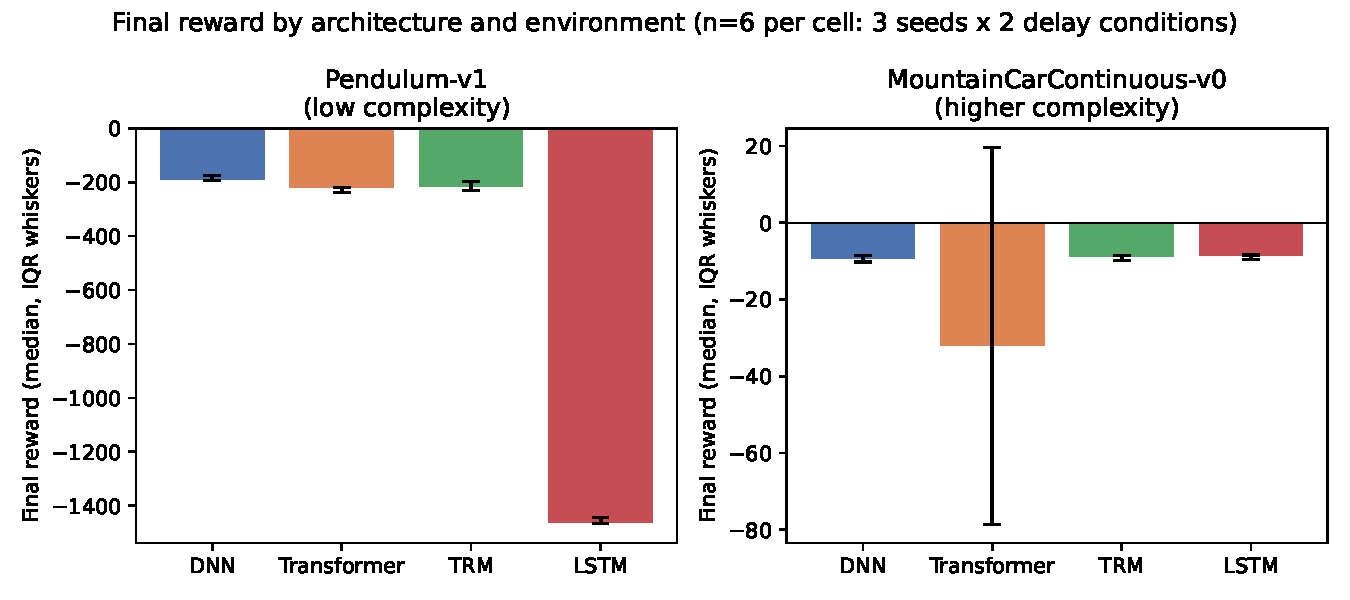
\includegraphics[width=0.95\textwidth]{figures/fig1_reward_by_arch_env.pdf}
\caption{Final reward by architecture and environment.}
\end{figure}

\begin{figure}[h]
\centering
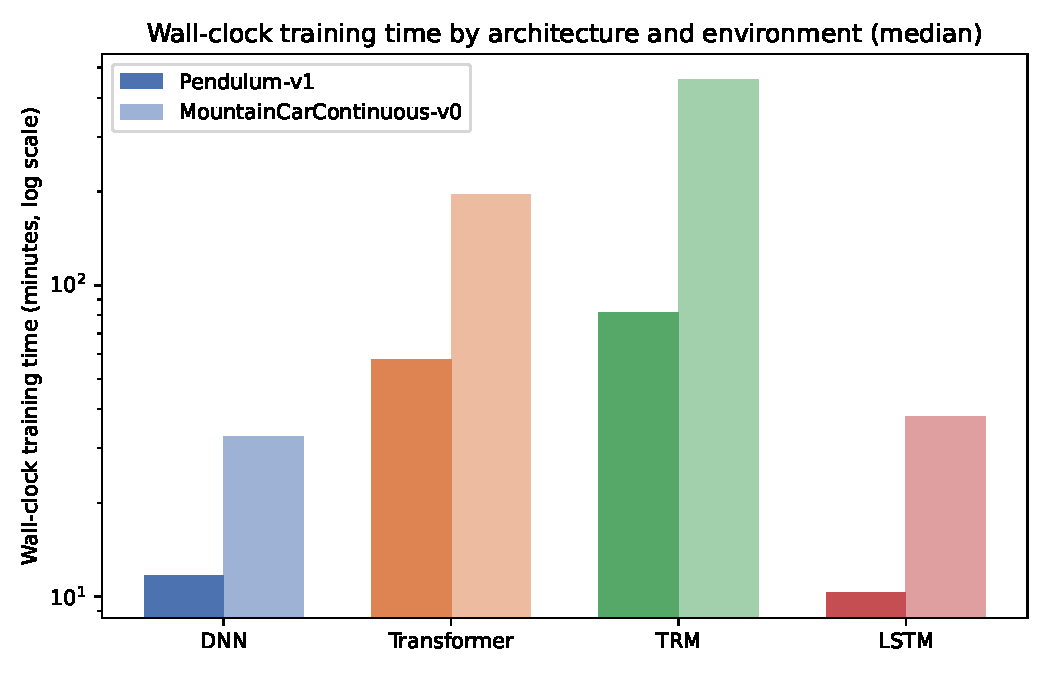
\includegraphics[width=0.75\textwidth]{figures/fig2_wallclock_by_arch_env.pdf}
\caption{Wall-clock training time by architecture and environment (median, log scale).}
\end{figure}

\textbf{Primary pre-registered test} (TRM vs.\ DNN, TRM vs.\ Transformer; pooled one-sided sign test, $n=6$ per cell):

\begin{table}[h]
\centering
\caption{Pre-registered primary comparison.}
\begin{tabular}{llrr}
\toprule
Comparison & Environment & TRM wins / total & one-sided $p$ \\
\midrule
TRM $-$ DNN & Pendulum-v1 & 0/6 & \textbf{0.0156} \\
TRM $-$ DNN & MountainCarContinuous-v0 & 3/6 & 0.656 \\
TRM $-$ Transformer & Pendulum-v1 & 3/6 & 0.656 \\
TRM $-$ Transformer & MountainCarContinuous-v0 & 4/6 & 0.344 \\
\bottomrule
\end{tabular}
\end{table}

On Pendulum-v1, TRM was significantly \textbf{worse} than DNN --- all 6 seed-pairs favored DNN ($p=0.0156$) --- a materially different result from the informal pilot's ``comparable reward'' characterization; the full 6-seed replication under this exact codebase shows a real, consistent gap. TRM vs.\ Transformer on Pendulum was an even 3/6 split (not significant).

On MountainCarContinuous-v0, neither comparison reached the pre-registered significance threshold in either direction: TRM vs.\ DNN was an exact 3/6 tie ($p=0.656$), and TRM vs.\ Transformer favored TRM 4/6 but fell short of significance ($p=0.344$).

\begin{figure}[h]
\centering
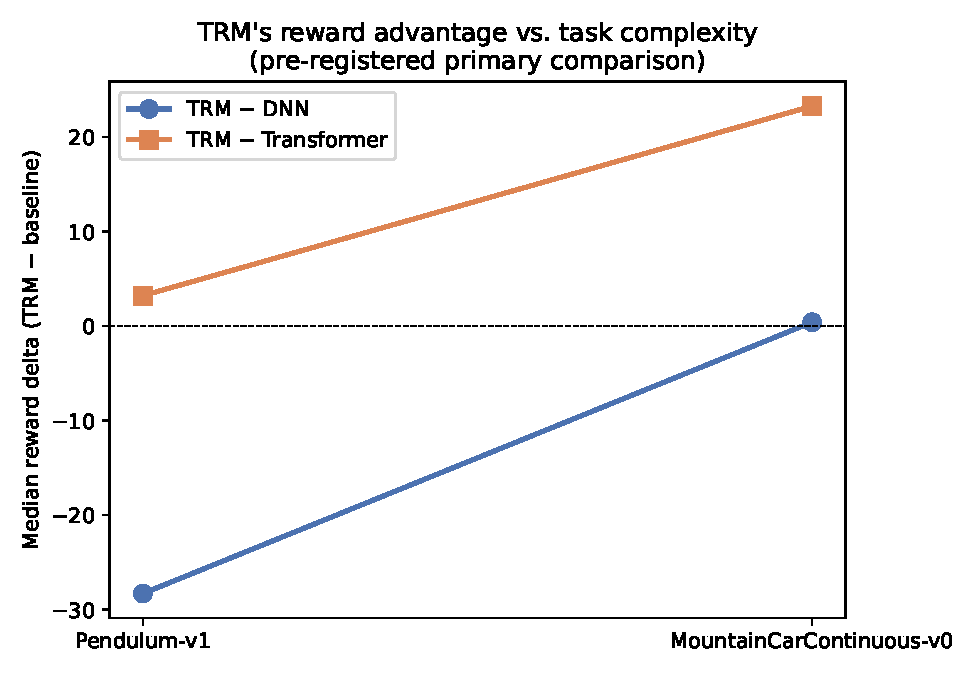
\includegraphics[width=0.7\textwidth]{figures/fig3_trm_advantage_trend.pdf}
\caption{TRM's reward advantage vs.\ task complexity (pre-registered primary comparison).}
\end{figure}

The median TRM-advantage delta moved from $-28.3$ (Pendulum) to $+0.4$ (MountainCarContinuous) vs.\ DNN, and from $+3.2$ to $+23.3$ vs.\ Transformer --- both monotonically increasing in the hypothesized direction, but neither rung reaches significance on the MountainCarContinuous cell, so this is reported as a \emph{directional} observation, not confirmatory evidence, per the pre-registered power statement (\S3).

\textbf{Wall-clock and parameter count.} TRM's wall-clock overhead relative to DNN \emph{grew} with task complexity: 7.0x on Pendulum-v1 (82.0 vs.\ 11.7 min) to 14.1x on MountainCarContinuous-v0 (457.3 vs.\ 32.5 min). Transformer's overhead grew more mildly (4.9x $\to$ 6.0x).

\begin{figure}[h]
\centering
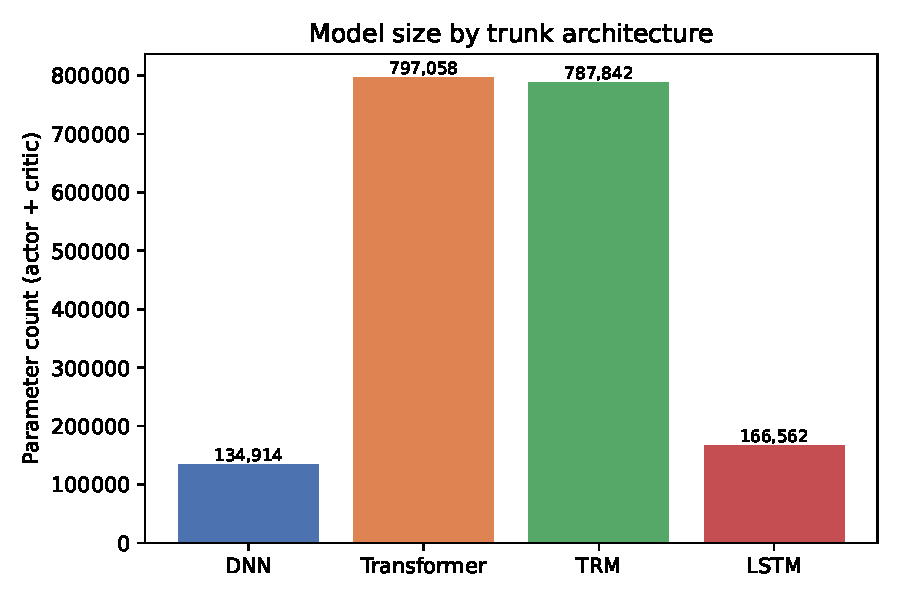
\includegraphics[width=0.6\textwidth]{figures/fig4_param_count.pdf}
\caption{Model size by trunk architecture.}
\end{figure}

TRM and Transformer have essentially the same parameter count ($\approx$5.84x and $\approx$5.91x DNN, respectively); LSTM is much closer to DNN in size ($\approx$1.23x DNN).

\textbf{Secondary/unplanned finding: LSTM failed to learn on Pendulum-v1.} Across all 6 seeds, LSTM's final reward (median $-1460.5$) matches an untrained/random policy, while it learned normally on MountainCarContinuous-v0 (median $-8.5$, on par with DNN and TRM). This produces a large, ``significant'' TRM-vs-LSTM gap on Pendulum (6/6, $p=0.0156$) that collapses on MountainCarContinuous (1/6, $p=0.109$) --- an artifact of the LSTM anomaly, not evidence about TRM's mechanism (see \S\ref{sec:limitations}).

\section{Discussion}

\textbf{On the primary hypothesis (H1 vs.\ H0).} The evidence is a genuine, bounded middle ground. TRM did not merely fail to show an advantage on the simple task --- it was significantly worse than DNN on Pendulum-v1 in this full replication. That deficit closed to a statistical tie on MountainCarContinuous-v0, moving in the pre-registered direction for both comparisons, but never reaching significance in TRM's favor. \textbf{We report the specific horizon/sparsity threshold prediction as falsified --- MountainCarContinuous-v0 does not produce a significant TRM advantage --- while the general hypothesis remains open}, since the trend is directionally consistent with it and a higher-complexity rung (Phase 2) has not been tested. This is exactly the kind of bounded, non-definitive outcome this project's research boundaries treat as valid.

\textbf{On cost.} TRM's wall-clock cost is not staying flat relative to DNN --- it roughly doubled in relative terms (7.0x $\to$ 14.1x) over one rung. Even under the best-case reading of the reward trend, this experiment gives no indication the \emph{rate} of cost growth is bounded.

\textbf{On the LSTM comparison.} Inconclusive, because the LSTM result on Pendulum-v1 is itself anomalous rather than a clean baseline (\S\ref{sec:limitations}). On MountainCarContinuous-v0 --- where LSTM learned normally --- its reward was statistically indistinguishable from TRM's and DNN's, giving no evidence that depth-of-refinement (TRM) or breadth-of-memory (LSTM, in this scoped stateless-per-call form) does meaningfully more than a plain MLP at this task's complexity.

\textbf{Next steps.} Per the pre-committed Phase 2 plan (\S\ref{sec:method}), the natural continuation is BipedalWalker-v3 --- a dimensionality/coupling axis rather than horizon/sparsity --- to test whether the observed trend continues, plateaus, or reverses. Phase 2 has \textbf{not} been run; this draft stops at Phase 1 pending author review. The Pendulum-v1 replication gap (TRM significantly worse here vs.\ ``comparable'' in the informal pilot) is itself worth understanding before over-interpreting the MountainCarContinuous trend --- possible explanations include seed count, training-budget/hyperparameter drift, or genuine configuration sensitivity; not investigated further here per explicit scoping direction during this project.

\section{Limitations}
\label{sec:limitations}

\begin{itemize}
  \item \textbf{Single environment carrying the core empirical test.} Three rounds of hypothesis-stage peer review converged on this as the primary limitation: the Phase 1 core claim rests substantially on one sparse-reward environment (MountainCarContinuous-v0) with a statistically modest sample size ($n=6$ paired comparisons per architecture-pair, minimum achievable $p \approx 0.03$). A clean result at this scale is evidence for or against the \emph{specific pre-registered threshold prediction}, not a fully general claim about complexity-scaling --- that requires the pre-committed Phase 2 (BipedalWalker-v3) and, contingent on infrastructure, a MuJoCo rung.
  \item \textbf{Complexity axes are not independently manipulated.} The three originally-proposed complexity axes (state/action dimensionality, horizon, dynamics coupling) are realized by swapping whole environments rather than holding two axes fixed while varying the third; per-environment axis values are reported descriptively, but attributing an observed effect to one axis specifically is not supported by this design.
  \item \textbf{The LSTM trunk is a scoped mechanistic control, not a full recurrent policy.} It processes the same per-call augmented observation as the other trunks, with no hidden state persisted across environment steps --- a deliberate scoping choice to avoid redesigning the training loop's replay-buffer sampling, stated here so the depth-of-refinement/breadth-of-memory contrast is not overclaimed as a like-for-like replication of \citet{bakker2007recurrent}'s cross-episode recurrent policy. A secondary, unplanned observation from Phase 1: the LSTM trunk failed to learn on Pendulum-v1 across all 6 seeds (reward matching an untrained policy) while learning normally on MountainCarContinuous-v0 --- reproducible, not an outlier, but not root-caused within this project's scope (a plausible but unverified explanation is gate-saturation sensitivity to Pendulum's larger angular-velocity range). This is noted as an open aside; it is secondary to the primary TRM-vs-DNN/Transformer comparison and was not chased further so as not to divert effort from the main hypothesis test.
  \item \textbf{Algorithm and hyperparameters fixed to the original pilot's choice (DDPG).} The finding, whichever direction it points, is scoped to this off-policy algorithm and its default hyperparameters; TD3/SAC or different learning rates/network widths are not tested here.
\end{itemize}

\section{Conclusion}

Under model-free, delay-robust continuous control with observation augmentation, TRM's recursive weight-tied trunk was \textbf{significantly worse} than a memoryless DNN on the low-complexity task (Pendulum-v1, $p=0.0156$, 6/6 seeds) --- a materially different picture than an earlier informal pilot's ``comparable reward'' characterization. On a higher-complexity task (MountainCarContinuous-v0, $\sim$5x longer horizon, sparse reward), that deficit closed to a statistical tie against both DNN and Transformer, moving in the direction the pre-registered hypothesis predicted, but never reaching significance in TRM's favor. We therefore report the specific threshold prediction tested here as \textbf{falsified} --- this complexity increase does not produce a statistically significant TRM advantage --- while treating the general complexity-scaling hypothesis as still open, since the direction of the effect does not rule it out at a higher rung. Meanwhile, TRM's wall-clock cost relative to DNN \textbf{grew} with complexity (7.0x $\to$ 14.1x), so even the best-case reading of the trend gives no evidence that TRM's cost is bounded as tasks get harder. At the evidence level established here, TRM's recursive mechanism does not yet earn its overhead in this setting; whether it does so at higher complexity (Phase 2: BipedalWalker-v3, a dimensionality/coupling axis rather than horizon/sparsity) remains an open, pre-committed next step.

\bibliographystyle{plainnat}
\begin{thebibliography}{9}

\bibitem[Jain and Linares(2025)]{jainlinares2025trc}
Jain, A. and Linares, R. (2025).
\newblock Tiny Recursive Control: Iterative Reasoning for Efficient Optimal Control.
\newblock \emph{arXiv:2512.16824}.

\bibitem[Wijayatunga and Armellin(2026)]{wijayatunga2026trmpl}
Wijayatunga, M. and Armellin, R. (2026).
\newblock Tiny Recursive Models for Solving the J2-Perturbed Lambert Problem.
\newblock \emph{arXiv:2606.00895}.

\bibitem[Jolicoeur-Martineau(2025)]{jolicoeurmartineau2025trm}
Jolicoeur-Martineau, A. (2025).
\newblock Less is More: Recursive Reasoning with Tiny Networks.
\newblock \emph{arXiv:2510.04871}.

\bibitem[Katsikopoulos and Engelbrecht(2003)]{katsikopoulos2003delayed}
Katsikopoulos, K.~V. and Engelbrecht, S.~E. (2003).
\newblock Markov decision processes with delays and asynchronous cost collection.
\newblock \emph{IEEE Transactions on Automatic Control}, 48(4):568--574.

\bibitem[Ramstedt et~al.(2021)]{ramstedt2021rlrandomdelays}
Ramstedt, S., Bouteiller, Y., Beltrame, G., Pal, C., and Binas, J. (2021).
\newblock Reinforcement Learning with Random Delays.
\newblock \emph{ICLR 2021}, \emph{arXiv:2010.02966}.

\bibitem[Morad et~al.(2023)]{morad2023popgym}
Morad, S., Kortvelesy, R., Bettini, M., Liwicki, S., and Prorok, A. (2023).
\newblock POPGym: Benchmarking Partially Observable Reinforcement Learning.
\newblock \emph{arXiv:2303.01859}.

\bibitem[Bakker(2007)]{bakker2007recurrent}
Bakker, B. (2007).
\newblock Solving Deep Memory POMDPs with Recurrent Policy Gradients.
\newblock \emph{ICANN 2007}.

\end{thebibliography}

\end{document}
